\documentclass{article}

\usepackage{amsmath}
\usepackage{graphicx}
\usepackage{hyperref}

\begin{document}

\title{Goddard Rocket Problem}
\author{Geoffrey Ulman\\
        Homework 5\\
        CSI747}
\date{October 2012}
\maketitle

\section{Physics Equations}\label{Physics Equations}

Let \(h(t)\) describe the height of a rocket at time \(t\), \(v(t)\) describe its velocity, \(a(t)\) its acceleration, \(T(t)\) the thrust produced by its engine, \(m(t)\) its mass, and \(R(t)\) the force of air resistance acting on the rocket.

\begin{eqnarray}\label{eq1}
v(t) = \frac{dh(t)}{dt} \nonumber \\
a(t) = \frac{dv(t)}{dt}
\end{eqnarray}

Equation \ref{eq1} describes the relationship between \(h(t)\), \(v(t)\), and \(a(t)\) (which comes from basic calculus and the definition of velocity and acceleration).

\begin{equation}\label{eq2}
m(t)a(t) = T(t) - R(t) - m(t)g
\end{equation}

Newton's second law states that the net force on an object is equal to its mass times its acceleration. This allows us to describe the relationship between the gravitational, thrust, and air resistance forces acting on the rocket (where \(g\) is the acceleration due to gravity). This relationship is described by equation \ref{eq2}.

\begin{equation}\label{eq3}
R(t) = \sigma v(t)^2 e^{\frac{-h(t)}{d}}
\end{equation}

The force of air resistance \(R(t)\) is proportional to the square of the velocity of the rocket with a proportionality constant \(\sigma\) and decays exponentially with height \(h(t)\) (\(d\) is an air density adjustment parameter). This force is described by equation \ref{eq3}.

\begin{equation}\label{eq4}
T(t) = -c \frac{dm(t)}{dt}
\end{equation}

Finally, the overall thrust of the rocket is inversely proportional to the rate of change in the rocket's mass (as fuel is consumed) with proportionality constant \(c\). This relationship is described by equation \ref{eq4}.

\section{Discretization}\label{Discretization}

To model the above equations in AMPL, the problem was divided into \(n\) time steps with variable \(tf\) representing the unknown final time. Velocity was modeled as the difference in rocket height at adjacent steps divided by the time difference between steps. Acceleration was similarly modeled and indexed such that indices for height and acceleration corresponded to values for the same time step. Velocity values were averaged to arrive at velocity values corresponding to the same time steps as the height and acceleration values.

\section{AMPL Model}\label{AMPL Model}

\begin{verbatim}

reset;

model;

param g  := 32.174; # in ft/s^2 
param Tmax  := 200; #maximum thrust capable of rocket 
param sigma := 5.4915e-5; #air resistance parameter 
param c  := 1580.9425; #thrust coeff 
param d  := 23800; #air density adjustment parameter 
param m0 := 3; #initial mass (measured in units) 
param mempty := 0.01;# mass of the rocket without the fuel

# discretization
param n := 300;

# final moment of time
var tf >= 80, <=220, := 200;

# height of rocket
var h {j in 0..n} >= 0;

# velocity of rocket
var v {j in 1..n} = ( h[j] - h[j-1] ) / ( tf / n );

# average velocity at h[1] through h[n-1]
var v_avg {j in 1..n-1} = ( v[j] + v[j+1] ) / 2;

# acceleration of rocket
var a {j in 1..n-1} = ( v[j+1] - v[j] ) / ( tf / n );

# thrust of rocket
var T {j in 0..n} >= 0, <= Tmax;

# mass of rocket
var m {j in 0..n} >= mempty, <= m0;

# derivative of mass with respect to time
var d_m {j in 1..n} = ( m[j] - m[j-1] ) / ( tf / n );

# average derivative of mass at m[1] through m[n-1]
var d_m_avg {j in 1..n-1} = ( d_m[j] + d_m[j+1] ) / 2;

# air resistance acting against rocket
var R {j in 0..n};

# maximize the final altitude of the rocket
maximize altitude: h[n];

# constrained by Newton's second law (F=MA)
s.t. newton {j in 1..n-1}: m[j] * a[j] = T[j] - R[j] - m[j] * g;

# where air reistance is defined as follows
s.t. air_resistance {j in 1..n-1}: R[j] = sigma *
                                          ( v_avg[j] )^2 *
                                          exp( -h[j] / d );

# trust of the rocket is proportional to the
# amount of fuel being burned
s.t. thrust {j in 1..n-1}: T[j] = -c * d_m_avg[j];

# initial conditions
s.t. initial_height: h[0] = 0;
s.t. initial_velocity: v[1] = 0;
s.t. initial_mass: m[0] = m0;

s.t. neg_d_m {j in 1..n}: d_m[j] <= 0;
s.t. neg_d_m_avg {j in 1..n-1}: d_m_avg[j] <= 0;

option solver loqo;

option loqo_options "iterlim=20000";

solve;

display tf;
display altitude;
display a;
display v;
display h;
display m;
display T;
display R;

\end{verbatim}

\section{AMPL Results}\label{AMPL Results}

\begin{figure}
\centering
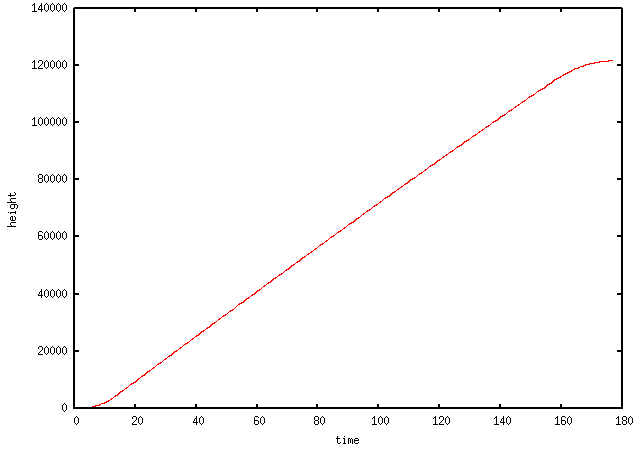
\includegraphics[width=0.9\textwidth]{homework5a_height.png}
\caption{Rocket Height Over Time}
\vspace{2 cm}
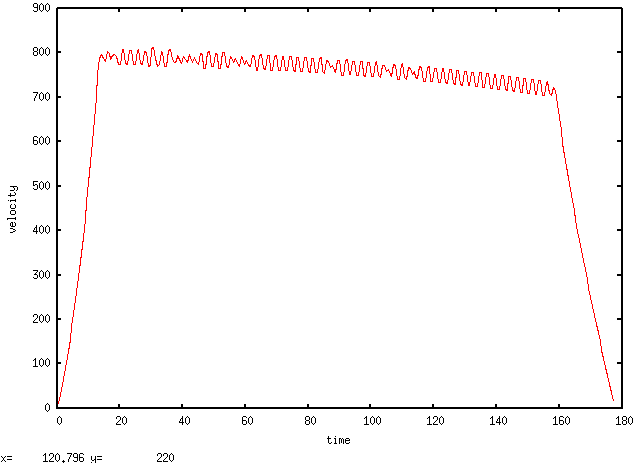
\includegraphics[width=0.9\textwidth]{homework5a_velocity.png}
\caption{Rocket Velocity Over Time}
\end{figure}

\begin{figure}
\centering
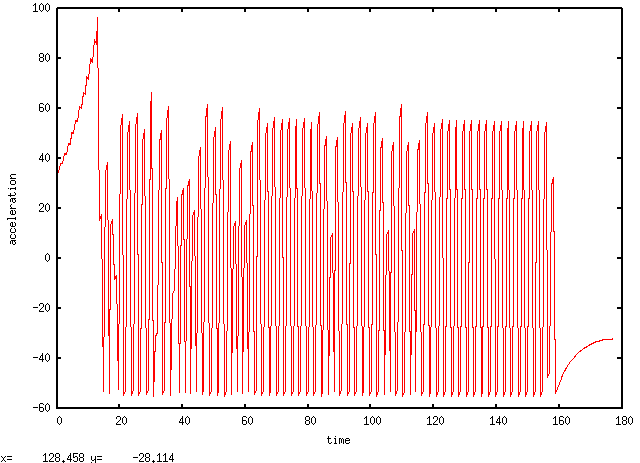
\includegraphics[width=0.9\textwidth]{homework5a_acceleration.png}
\caption{Rocket Acceleration Over Time}
\vspace{2 cm}
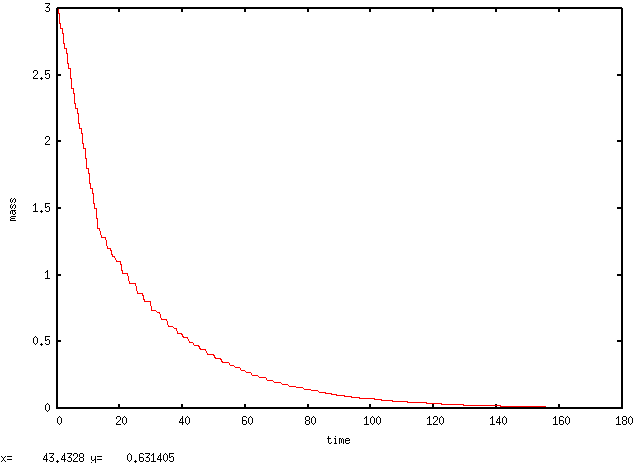
\includegraphics[width=0.9\textwidth]{homework5a_mass.png}
\caption{Rocket Mass Over Time}
\end{figure}

\begin{figure}
\centering
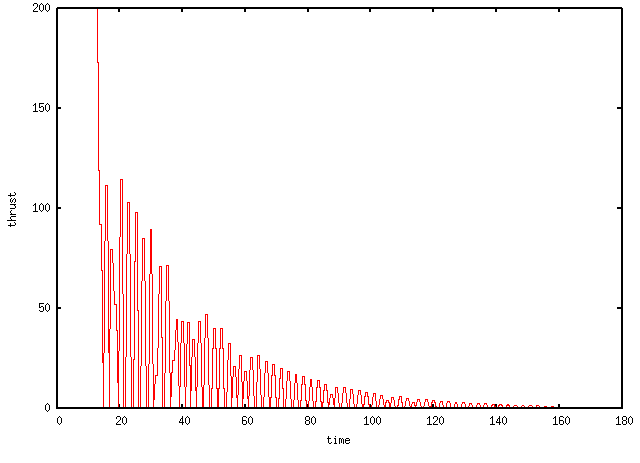
\includegraphics[width=0.9\textwidth]{homework5a_thrust.png}
\caption{Rocket Thrust Over Time}
\vspace{2 cm}
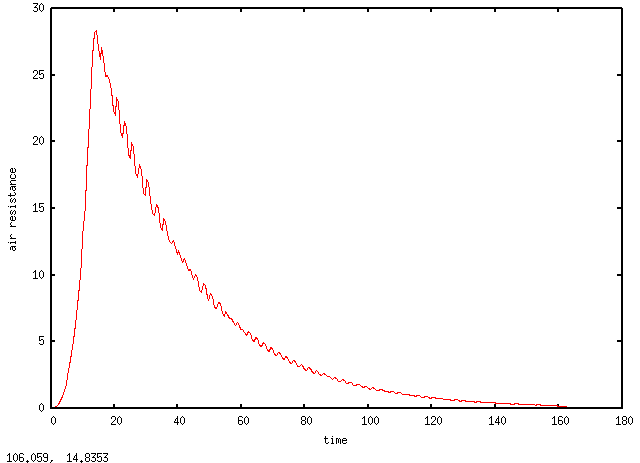
\includegraphics[width=0.9\textwidth]{homework5a_air_resistance.png}
\caption{Rocket Air Resistance Over Time}
\end{figure}

\scriptsize
\begin{verbatim}

*************************************************************

   NEOS Server Version 5.0
   Job#     : 309789
   Password : JPsdjLDC
   Solver   : nco:LOQO:AMPL
   Start    : 2012-09-27 21:55:12
   End      : 2012-09-27 21:56:21
   Host     : neos-1.chtc.wisc.edu

   Disclaimer:

   This information is provided without any express or
   implied warranty. In particular, there is no warranty
   of any kind concerning the fitness of this
   information  for any particular purpose.
*************************************************************
Job 309789 sent to neos-1.chtc.wisc.edu
password: JPsdjLDC
---------- Begin Solver Output -----------
Executing /opt/neos/Drivers/loqo-ampl/loqo-driver.py at time: 2012-09-27 21:55:12.793343
File exists
You are using the solver loqo.

%% YOUR COMMENTS %%%%%%%%%%%%%%%%%%%%%%%
Job 1
%%%%%%%%%%%%%%%%%%%%%%%%%%%%%%%%%%%%%%%%
Executing AMPL.
processing data.
processing commands.

Presolve eliminates 3 constraints and 7 variables.
Substitution eliminates 1496 variables.
Adjusted problem:
1199 variables:
	601 nonlinear variables
	598 linear variables
1497 constraints, all nonlinear; 7176 nonzeros
	898 equality constraints
	599 inequality constraints
1 linear objective; 1 nonzero.

LOQO 6.07: iterlim=20000
LOQO 6.07: optimal solution (1019 iterations, 3065 evaluations)
primal objective 121642.9087
  dual objective 121642.908

tf = 177.751

altitude = 121643

a [*] :=
  1  34.4908     61 -54.9812    121  55.3808    181  46.3049    241 -52.9132
  2  37.9799     62 -14.0376    122 -54.8391    182 -54.7421    242  49.5761
  3  37.9428     63 -12.6346    123 -52.6532    183 -52.5334    243  54.8359
  4  41.7725     64  21.5862    124  50.4155    184  55.3291    244 -55.2457
  5  41.6826     65  24.4341    125  55.9088    185  61.362     245 -52.9259
  6  45.8968     66 -53.599     126 -54.8641    186 -55.2606    246  49.5436
  7  45.7339     67  24.8261    127 -52.6739    187 -52.9947    247  54.7923
  8  50.3841     68  27.8974    128  50.0035    188  42.0189    248 -55.2656
  9  50.1224     69 -53.5979    129  55.4458    189  46.5348    249 -52.9388
 10  55.2703     70  28.3982    130 -54.8531    190 -54.5434    250  49.5176
 11  54.8769     71  31.7508    131 -52.6623    191   9.4839    251  54.7558
 12  60.5974     72 -53.893     132  50.6188    192  11.593     252 -55.2867
 13  60.0304     73  16.6597    133  56.1308    193 -53.2488    253 -52.9524
 14  66.4166     74  19.178     134 -54.8996    194  42.4716    254  49.4705
 15  65.6234     75 -53.2142    135 -52.7021    195  47.0391    255  54.6955
 16  72.7936     76  39.8399    136  49.1969    196 -54.8487    256 -55.3069
 17  71.707      77  44.2202    137  54.5393    197 -52.6185    257 -52.9651
 18  79.8158     78 -54.4819    138 -54.8191    198  52.7318    258  49.4817
 19  78.3505     79 -52.3482    139 -52.628     199  58.4261    259  54.6998
 20  87.6055     80  55.32      140  52.5651    200 -55.1375    260 -55.3319
 21  85.6511     81  61.4354    141  58.3045    201 -52.8737    261 -52.9819
 22  96.3405     82 -54.9405    142 -55.0459    202  48.7264    262  49.3232
 23  15.0062     83 -52.7585    143 -52.8294    203  53.952     263  54.515
 24  17.4412     84  47.0728    144  44.1295    204 -55.0436    264 -47.7026
 25 -53.2484     85  52.2062    145  48.9015    205 -52.7863    265 -45.6775
 26  34.4574     86 -54.6479    146 -54.5123    206  50.2607    266  29.0435
 27  38.334      87 -52.4948    147   7.96878   207  55.6551    267  32.302
 28 -54.0422     88  54.3807    148  10.0187    208 -55.1007    268 -54.1401
 29  13.1391     89  60.3784    149 -53.0946    209 -52.8339    269 -51.9066
 30  15.462      90 -55.0173    150  43.5646    210  49.6318    270 -49.907
 31  -8.31443    91 -52.8248    151  48.2832    211  54.9489    271 -48.1112
 32  -6.78914    92  42.1946    152 -54.7379    212 -55.0998    272 -46.4941
 33 -52.505      93  46.7927    153 -52.5481    213 -52.8295    273 -45.0343
 34  51.8809     94 -54.3005    154  52.8187    214  49.8387    274 -43.7136
 35  57.5928     95  12.5371    155  58.5727    215  55.1737    275 -42.5165
 36 -54.7749     96  14.8266    156 -55.0029    216 -55.122     276 -41.4298
 37 -52.6215     97 -53.2657    157 -52.7834    217 -52.8456    277 -40.4418
 38  49.255      98  35.1089    158  48.8326    218  49.7228    278 -39.5426
 39  54.6549     99  39.0223    159  54.117     219  55.0387    279 -38.7237
 40 -54.6701    100 -54.1414    160 -54.8955    220 -55.1359    280 -37.9774
 41 -52.5266    101  12.7995    161 -52.6848    221 -52.8542    281 -37.2972
 42  52.3692    102  15.0944    162  50.9183    222  49.7297    282 -36.6774
 43  58.1392    103 -53.1391    163  56.4399    223  55.0403    283 -36.1128
 44 -54.8438    104  41.767     164 -54.9852    224 -55.1537    284 -35.599
 45 -52.6816    105  46.3286    165 -52.7628    225 -52.8661    285 -35.1322
 46  46.3965    106 -54.5883    166  48.848     226  49.689     286 -34.7088
 47  51.4661    107 -52.4345    167  54.1253    227  54.9888    287 -34.3259
 48 -54.4899    108  53.8659    168 -54.8859    228 -55.1707    288 -33.9807
 49 -52.363     109  59.7831    169 -52.6714    229 -52.8772    289 -33.671
 50  59.4803    110 -54.9264    170  52.6674    230  49.6655    290 -33.3946
 51  66.1624    111 -52.7363    171  58.3915    231  54.9562    291 -33.1499
 52 -55.3019    112  48.7278    172 -55.14      232 -55.1888    292 -32.9351
 53 -31.17      113  54.0344    173 -52.8964    233 -52.889     293 -32.749
 54 -29.7758    114 -54.7904    174  43.3234    234  49.6349    294 -32.5904
 55  46.2286    115 -52.6128    175  47.986     235  54.9153    295 -32.4584
 56  51.2806    116  50.9256    176 -54.5419    236 -55.2071    296 -32.3521
 57 -54.5854    117  56.484     177   9.17056   237 -52.9009    297 -32.271
 58 -52.4467    118 -54.8597    178  11.27      238  49.6058    298 -32.2145
 59  54.7809    119 -52.6733    179 -53.221     239  54.8761    299 -32.1824
 60  60.8428    120  49.9401    180  41.7938    240 -55.2261
;

v [*] :=
  1   0          61 822.575     121 775.101     181 759.588     241 731.985
  2  20.4359     62 789.998     122 807.915     182 787.024     242 700.634
  3  42.9391     63 781.681     123 775.422     183 754.589     243 730.008
  4  65.4203     64 774.195     124 744.225     184 723.463     244 762.498
  5  90.1707     65 786.985     125 774.097     185 756.245     245 729.765
  6 114.868      66 801.462     126 807.223     186 792.603     246 698.406
  7 142.062      67 769.704     127 774.716     187 759.86      247 727.761
  8 169.159      68 784.414     128 743.506     188 728.461     248 760.226
  9 199.012      69 800.943     129 773.133     189 753.357     249 727.481
 10 228.71       70 769.186     130 805.985     190 780.929     250 696.114
 11 261.457      71 786.012     131 773.484     191 748.612     251 725.453
 12 293.972      72 804.825     132 742.282     192 754.231     252 757.896
 13 329.876      73 772.893     133 772.274     193 761.1       253 725.139
 14 365.444      74 782.764     134 805.531     194 729.55      254 693.764
 15 404.797      75 794.127     135 773.003     195 754.715     255 723.076
 16 443.679      76 762.597     136 741.777     196 782.585     256 755.483
 17 486.809      77 786.203     137 770.926     197 750.087     257 722.714
 18 529.296      78 812.403     138 803.241     198 718.911     258 691.332
 19 576.587      79 780.123     139 770.761     199 750.155     259 720.65
 20 623.01       80 749.106     140 739.578     200 784.772     260 753.06
 21 674.916      81 781.883     141 770.723     201 752.103     261 720.275
 22 725.665      82 818.284     142 805.269     202 720.775     262 688.883
 23 782.747      83 785.732     143 772.654     203 749.646     263 718.107
 24 791.638      84 754.472     144 741.352     204 781.613     264 750.408
 25 801.972      85 782.363     145 767.499     205 748.999     265 722.144
 26 770.422      86 813.295     146 796.474     206 717.723     266 695.08
 27 790.838      87 780.916     147 764.175     207 747.503     267 712.288
 28 813.551      88 749.813     148 768.896     208 780.478     268 731.427
 29 781.531      89 782.033     149 774.833     209 747.831     269 699.349
 30 789.316      90 817.808     150 743.374     210 716.527     270 668.594
 31 798.477      91 785.21      151 769.186     211 745.934     271 639.024
 32 793.551      92 753.911     152 797.794     212 778.491     272 610.518
 33 789.528      93 778.911     153 765.362     213 745.844     273 582.97
 34 758.419      94 806.636     154 734.227     214 714.543     274 556.287
 35 789.159      95 774.463     155 765.522     215 744.072     275 530.387
 36 823.283      96 781.891     156 800.226     216 776.763     276 505.196
 37 790.828      97 790.676     157 767.637     217 744.103     277 480.648
 38 759.65       98 759.116     158 736.363     218 712.792     278 456.686
 39 788.834      99 779.918     159 765.296     219 742.253     279 433.257
 40 821.217     100 803.039     160 797.361     220 774.863     280 410.313
 41 788.825     101 770.96      161 764.835     221 742.195     281 387.812
 42 757.702     102 778.544     162 733.619     222 710.879     282 365.713
 43 788.731     103 787.487     163 763.788     223 740.344     283 343.982
 44 823.179     104 756.002     164 797.229     224 772.955     284 322.585
 45 790.684     105 780.749     165 764.65      225 740.277     285 301.492
 46 759.47      106 808.199     166 733.388     226 708.953     286 280.676
 47 786.96      107 775.855     167 762.331     227 738.394     287 260.111
 48 817.454     108 744.788     168 794.4       228 770.975     288 239.773
 49 785.168     109 776.703     169 761.88      229 738.287     289 219.639
 50 754.143     110 812.125     170 730.672     230 706.957     290 199.689
 51 789.385     111 779.581     171 761.878     231 736.384     291 179.903
 52 828.587     112 748.335     172 796.475     232 768.945     292 160.261
 53 795.82      113 777.206     173 763.804     233 736.246     293 140.747
 54 777.352     114 809.222     174 732.463     234 704.909     294 121.343
 55 759.71      115 776.758     175 758.132     235 734.318     295 102.033
 56 787.1       116 745.585     176 786.564     236 766.855     296  82.8016
 57 817.484     117 775.758     177 754.248     237 734.145     297  63.6329
 58 785.142     118 809.225     178 759.681     238 702.801     298  44.5122
 59 754.067     119 776.721     179 766.359     239 732.192     299  25.425
 60 786.525     120 745.512     180 734.825     240 764.707     300   6.35686
;

h [*] :=
  0      0             101  40835.5           202  86735.3
  1      1.75884e-14   102  41296.8           203  87179.5
  2     12.1083        103  41763.3           204  87642.6
  3     37.5499        104  42211.3           205  88086.4
  4     76.3116        105  42673.9           206  88511.6
  5    129.738         106  43152.7           207  88954.5
  6    197.797         107  43612.4           208  89417
  7    281.969         108  44053.7           209  89860
  8    382.197         109  44513.9           210  90284.6
  9    500.112         110  44995.1           211  90726.6
 10    635.623         111  45457             212  91187.8
 11    790.538         112  45900.4           213  91629.7
 12    964.717         113  46360.9           214  92053.1
 13   1160.17          114  46840.4           215  92494
 14   1376.7           115  47300.6           216  92954.2
 15   1616.54          116  47742.4           217  93395.1
 16   1879.42          117  48202             218  93817.4
 17   2167.86          118  48681.5           219  94257.2
 18   2481.47          119  49141.7           220  94716.3
 19   2823.1           120  49583.4           221  95156.1
 20   3192.23          121  50042.6           222  95577.3
 21   3592.12          122  50521.3           223  96015.9
 22   4022.08          123  50980.8           224  96473.9
 23   4485.86          124  51421.7           225  96912.5
 24   4954.91          125  51880.4           226  97332.6
 25   5430.08          126  52358.7           227  97770.1
 26   5886.55          127  52817.7           228  98226.9
 27   6355.13          128  53258.2           229  98664.3
 28   6837.16          129  53716.3           230  99083.2
 29   7300.22          130  54193.8           231  99519.5
 30   7767.89          131  54652.1           232  99975.1
 31   8240.99          132  55091.9           233 100411
 32   8711.17          133  55549.5           234 100829
 33   9178.97          134  56026.8           235 101264
 34   9628.34          135  56484.8           236 101718
 35  10095.9           136  56924.3           237 102153
 36  10583.7           137  57381.1           238 102570
 37  11052.3           138  57857             239 103004
 38  11502.4           139  58313.7           240 103457
 39  11969.8           140  58751.9           241 103890
 40  12456.3           141  59208.5           242 104306
 41  12923.7           142  59685.7           243 104738
 42  13372.7           143  60143.5           244 105190
 43  13840             144  60582.7           245 105622
 44  14327.7           145  61037.5           246 106036
 45  14796.2           146  61509.4           247 106467
 46  15246.2           147  61962.2           248 106918
 47  15712.5           148  62417.7           249 107349
 48  16196.8           149  62876.8           250 107761
 49  16662             150  63317.3           251 108191
 50  17108.9           151  63773             252 108640
 51  17576.6           152  64245.7           253 109070
 52  18067.5           153  64699.2           254 109481
 53  18539             154  65134.2           255 109909
 54  18999.6           155  65587.8           256 110357
 55  19449.8           156  66061.9           257 110785
 56  19916.1           157  66516.8           258 111195
 57  20400.5           158  66953.1           259 111622
 58  20865.7           159  67406.5           260 112068
 59  21312.5           160  67878.9           261 112495
 60  21778.5           161  68332.1           262 112903
 61  22265.9           162  68766.8           263 113328
 62  22733.9           163  69219.3           264 113773
 63  23197.1           164  69691.7           265 114201
 64  23655.8           165  70144.7           266 114613
 65  24122.1           166  70579.3           267 115035
 66  24597             167  71031             268 115468
 67  25053             168  71501.6           269 115882
 68  25517.8           169  71953.1           270 116279
 69  25992.3           170  72386             271 116657
 70  26448.1           171  72837.4           272 117019
 71  26913.8           172  73309.3           273 117364
 72  27390.7           173  73761.9           274 117694
 73  27848.6           174  74195.9           275 118008
 74  28312.4           175  74645.1           276 118307
 75  28782.9           176  75111.1           277 118592
 76  29234.7           177  75558             278 118863
 77  29700.6           178  76008.1           279 119120
 78  30181.9           179  76462.2           280 119363
 79  30644.2           180  76897.6           281 119592
 80  31088             181  77347.6           282 119809
 81  31551.3           182  77813.9           283 120013
 82  32036.1           183  78261             284 120204
 83  32501.7           184  78689.7           285 120383
 84  32948.7           185  79137.8           286 120549
 85  33412.2           186  79607.4           287 120703
 86  33894.1           187  80057.6           288 120845
 87  34356.8           188  80489.2           289 120975
 88  34801.1           189  80935.6           290 121094
 89  35264.4           190  81398.3           291 121200
 90  35749             191  81841.8           292 121295
 91  36214.2           192  82288.7           293 121379
 92  36660.9           193  82739.7           294 121450
 93  37122.4           194  83171.9           295 121511
 94  37600.4           195  83619.1           296 121560
 95  38059.2           196  84082.8           297 121598
 96  38522.5           197  84527.2           298 121624
 97  38991             198  84953.2           299 121639
 98  39440.8           199  85397.6           300 121643
 99  39902.9           200  85862.6
100  40378.7           201  86308.3
;

m [*] :=
  0 3            61 0.614182    122 0.18177     183 0.0549748   244 0.0159504
  1 3            62 0.614182    123 0.18177     184 0.0549748   245 0.0159504
  2 2.85009      63 0.596053    124 0.18177     185 0.0505433   246 0.0159504
  3 2.85009      64 0.596053    125 0.167784    186 0.0505433   247 0.0147303
  4 2.70018      65 0.562752    126 0.167784    187 0.0505433   248 0.0147303
  5 2.70018      66 0.562752    127 0.167784    188 0.0505433   249 0.0147303
  6 2.55027      67 0.562752    128 0.167784    189 0.0469646   250 0.0147303
  7 2.55027      68 0.530034    129 0.154923    190 0.0469646   251 0.0136036
  8 2.40035      69 0.530034    130 0.154923    191 0.0469646   252 0.0136036
  9 2.40035      70 0.530034    131 0.154923    192 0.044752    253 0.0136036
 10 2.25044      71 0.497777    132 0.154923    193 0.044752    254 0.0136036
 11 2.25044      72 0.497777    133 0.142977    194 0.044752    255 0.0125635
 12 2.10053      73 0.497777    134 0.142977    195 0.0415598   256 0.0125635
 13 2.10053      74 0.471828    135 0.142977    196 0.0415598   257 0.0125635
 14 1.95062      75 0.471828    136 0.142977    197 0.0415598   258 0.0125635
 15 1.95062      76 0.471828    137 0.132103    198 0.0415598   259 0.0116027
 16 1.80071      77 0.439133    138 0.132103    199 0.0382892   260 0.0116027
 17 1.80071      78 0.439133    139 0.132103    200 0.0382892   261 0.0116027
 18 1.6508       79 0.439133    140 0.132103    201 0.0382892   262 0.0116027
 19 1.6508       80 0.439133    141 0.121724    202 0.0382892   263 0.0107165
 20 1.50089      81 0.403801    142 0.121724    203 0.0353858   264 0.0107165
 21 1.50089      82 0.403801    143 0.121724    204 0.0353858   265 0.010654
 22 1.35098      83 0.403801    144 0.121724    205 0.0353858   266 0.010654
 23 1.35098      84 0.403801    145 0.112924    206 0.0353858   267 0.01
 24 1.28207      85 0.373727    146 0.112924    207 0.0326634   268 0.01
 25 1.28207      86 0.373727    147 0.112924    208 0.0326634   269 0.01
 26 1.28207      87 0.373727    148 0.107736    209 0.0326634   270 0.01
 27 1.19845      88 0.373727    149 0.107736    210 0.0326634   271 0.01
 28 1.19845      89 0.343886    150 0.107736    211 0.030165    272 0.01
 29 1.19845      90 0.343886    151 0.099974    212 0.030165    273 0.01
 30 1.13906      91 0.343886    152 0.099974    213 0.030165    274 0.01
 31 1.13906      92 0.343886    153 0.099974    214 0.030165    275 0.01
 32 1.10025      93 0.319535    154 0.099974    215 0.0278529   276 0.01
 33 1.10025      94 0.319535    155 0.0921056   216 0.0278529   277 0.01
 34 1.10025      95 0.319535    156 0.0921056   217 0.0278529   278 0.01
 35 1.01448      96 0.303789    157 0.0921056   218 0.0278529   279 0.01
 36 1.01448      97 0.303789    158 0.0921056   219 0.0257203   280 0.01
 37 1.01448      98 0.303789    159 0.0851203   220 0.0257203   281 0.01
 38 1.01448      99 0.283821    160 0.0851203   221 0.0257203   282 0.01
 39 0.937342    100 0.283821    161 0.0851203   222 0.0257203   283 0.01
 40 0.937342    101 0.283821    162 0.0851203   223 0.0237506   284 0.01
 41 0.937342    102 0.26981     163 0.0785357   224 0.0237506   285 0.01
 42 0.937342    103 0.26981     164 0.0785357   225 0.0237506   286 0.01
 43 0.863912    104 0.26981     165 0.0785357   226 0.0237506   287 0.01
 44 0.863912    105 0.250732    166 0.0785357   227 0.0219322   288 0.01
 45 0.863912    106 0.250732    167 0.0725798   228 0.0219322   289 0.01
 46 0.863912    107 0.250732    168 0.0725798   229 0.0219322   290 0.01
 47 0.800066    108 0.250732    169 0.0725798   230 0.0219322   291 0.01
 48 0.800066    109 0.23082     170 0.0725798   231 0.0202533   292 0.01
 49 0.800066    110 0.23082     171 0.0668692   232 0.0202533   293 0.01
 50 0.800066    111 0.23082     172 0.0668692   233 0.0202533   294 0.01
 51 0.733154    112 0.23082     173 0.0668692   234 0.0202533   295 0.01
 52 0.733154    113 0.213342    174 0.0668692   235 0.0187032   296 0.01
 53 0.733154    114 0.213342    175 0.0620729   236 0.0187032   297 0.01
 54 0.720915    115 0.213342    176 0.0620729   237 0.0187032   298 0.01
 55 0.720915    116 0.213342    177 0.0620729   238 0.0187032   299 0.01
 56 0.667675    117 0.196849    178 0.0591632   239 0.0172719   300 0.01
 57 0.667675    118 0.196849    179 0.0591632   240 0.0172719
 58 0.667675    119 0.196849    180 0.0591632   241 0.0172719
 59 0.667675    120 0.196849    181 0.0549748   242 0.0172719
 60 0.614182    121 0.18177     182 0.0549748   243 0.0159504
;

T [*] :=
  0   0              76  43.6199        152   1.12006e-07   228   3.90505e-08
  1 200              77  43.6199        153   1.10394e-07   229   3.92705e-08
  2 200              78   2.59397e-07   154  10.4975        230   2.23989
  3 200              79   2.52582e-07   155  10.4975        231   2.23989
  4 200              80  47.1369        156   6.04003e-08   232   3.79659e-08
  5 200              81  47.1369        157   6.25757e-08   233   3.82455e-08
  6 200              82   1.3069e-07    158   9.31912       234   2.06804
  7 200              83   1.34978e-07   159   9.31912       235   2.06804
  8 200              84  40.1217        160   7.19598e-08   236   3.71105e-08
  9 200              85  40.1217        161   7.0637e-08    237   3.73631e-08
 10 200              86   1.36636e-07   162   8.78474       238   1.90944
 11 200              87   1.33953e-07   163   8.78474       239   1.90944
 12 200              88  39.8127        164   6.80312e-08   240   3.62578e-08
 13 200              89  39.8127        165   7.02742e-08   241   3.65e-08
 14 200              90   1.96447e-07   166   7.94591       242   1.76302
 15 200              91   2.02812e-07   167   7.94591       243   1.76302
 16 200              92  32.4868        168   5.47209e-08   244   3.55242e-08
 17 200              93  32.4868        169   5.25897e-08   245   3.57933e-08
 18 200              94   5.67063e-08   170   7.61864       246   1.62782
 19 200              95  21.0065        171   7.61864       247   1.62782
 20 200              96  21.0065        172   1.01799e-07   248   3.48069e-08
 21 200              97   7.09747e-08   173   1.0452e-07    249   3.50218e-08
 22 200              98  26.6403        174   6.39881       250   1.5031
 23  91.9229         99  26.6403        175   6.39881       251   1.5031
 24  91.9229        100   6.8124e-08    176   2.28952e-08   252   3.43705e-08
 25   1.59622e-07   101  18.6918        177   3.88186       253   3.44363e-08
 26 111.558         102  18.6918        178   3.88186       254   1.38768
 27 111.558         103   5.1298e-08    179   2.42684e-08   255   1.38768
 28   1.60748e-07   104  25.4528        180   5.58781       256   3.32555e-08
 29  79.2336        105  25.4528        181   5.58781       257   3.49372e-08
 30  79.2336        106   1.9061e-07    182   7.42463e-08   258   1.28188
 31  51.79          107   1.86792e-07   183   7.02909e-08   259   1.28188
 32  51.79          108  26.5651        184   5.91221       260   3.32131e-08
 33   2.20653e-07   109  26.5651        185   5.91221       261   2.46993e-08
 34 114.421         110   9.37424e-08   186   6.66345e-08   262   1.18218
 35 114.421         111   9.61772e-08   187   7.12126e-08   263   1.18218
 36   2.52001e-07   112  23.3178        188   4.77438       264   0.0834388
 37   2.54864e-07   113  23.3178        189   4.77438       265   0.0834389
 38 102.911         114   1.17822e-07   190   2.07533e-08   266   0.872522
 39 102.911         115   1.17242e-07   191   2.95194       267   0.872522
 40   2.22368e-07   116  22.0032        192   2.95194       268   4.93958e-09
 41   2.20905e-07   117  22.0032        193   1.8363e-08    269   5.10682e-09
 42  97.9646        118   9.94938e-08   194   4.25879       270   1.03763e-09
 43  97.9646        119   1.00543e-07   195   4.25879       271   4.81504e-10
 44   2.83143e-07   120  20.1167        196   1.04177e-07   272   2.40862e-10
 45   2.89961e-07   121  20.1167        197   1.02963e-07   273   1.66305e-10
 46  85.1795        122   1.0065e-07    198   4.36334       274   1.16752e-10
 47  85.1795        123   1.00758e-07   199   4.36334       275   8.82946e-11
 48   1.49964e-07   124  18.6601        200   3.47544e-08   276   6.80882e-11
 49   1.41774e-07   125  18.6601        201   3.87442e-08   277   5.51642e-11
 50  89.2685        126   9.54483e-08   202   3.8735        278   4.57333e-11
 51  89.2685        127   9.62284e-08   203   3.8735        279   3.88575e-11
 52   2.52045e-06   128  17.1575        204   5.48914e-08   280   3.37204e-11
 53  16.3277        129  17.1575        205   5.24598e-08   281   3.03373e-11
 54  16.3277        130   8.96435e-08   206   3.63203       282   2.62638e-11
 55  71.0291        131   8.96162e-08   207   3.63203       283   2.37315e-11
 56  71.0291        132  15.9375        208   4.1391e-08    284   2.14592e-11
 57   2.20418e-07   133  15.9375        209   4.31297e-08   285   1.97668e-11
 58   2.0878e-07    134   9.30949e-08   210   3.33323       286   1.8115e-11
 59  71.3653        135   9.43491e-08   211   3.33323       287   1.69657e-11
 60  71.3653        136  14.5076        212   4.53868e-08   288   1.5958e-11
 61   2.0525e-07    137  14.5076        213   4.48604e-08   289   1.51184e-11
 62  24.1863        138   7.44361e-08   214   3.08451       290   1.43405e-11
 63  24.1863        139   7.34679e-08   215   3.08451       291   1.36544e-11
 64  44.4283        140  13.8469        216   4.15423e-08   292   1.33991e-11
 65  44.4283        141  13.8469        217   4.22204e-08   293   1.28409e-11
 66   9.59333e-08   142   1.17962e-07   218   2.84527       294   1.30418e-11
 67  43.6497        143   1.20413e-07   219   2.84527       295   1.25552e-11
 68  43.6497        144  11.7394        220   4.15175e-08   296   1.36427e-11
 69   7.64311e-08   145  11.7394        221   4.1588e-08    297   1.30553e-11
 70  43.0345        146   3.45708e-08   222   2.62782       298   1.68047e-11
 71  43.0345        147   6.92141       223   2.62782       299   1.59833e-11
 72   1.01167e-07   148   6.92141       224   3.98584e-08   300   0
 73  34.619         149   3.42536e-08   225   4.02227e-08
 74  34.619         150  10.356         226   2.42589
 75   6.64194e-08   151  10.356         227   2.42589
;

R [*] :=
  0  0              76  9.64175       152  2.2558        228  0.504369
  1  0.00573347     77 10.0727        153  2.03688       229  0.454066
  2  0.0551119      78  9.79612       154  2.00042       230  0.444971
  3  0.160946       79  8.85914       155  2.1392        231  0.47522
  4  0.331289       80  8.71549       156  2.10267       232  0.466124
  5  0.574029       81  9.33737       157  1.89824       233  0.419546
  6  0.898772       82  9.19314       158  1.85796       234  0.411145
  7  1.31408        83  8.31205       159  1.974         235  0.439197
  8  1.83129        84  8.12173       160  1.93406       236  0.430793
  9  2.45939        85  8.58648       161  1.74589       237  0.387659
 10  3.21159        86  8.39913       162  1.7119        238  0.379901
 11  4.09698        87  7.59444       163  1.82539       239  0.405919
 12  5.1308         88  7.46488       164  1.79149       240  0.398154
 13  6.32166        89  7.9853        165  1.61696       241  0.358207
 14  7.6871         90  7.85547       166  1.58279       242  0.351042
 15  9.23445        91  7.10152       167  1.68232       243  0.375178
 16 10.9839         92  6.91255       168  1.64842       244  0.368003
 17 12.9405         93  7.25424       169  1.4877        245  0.331002
 18 15.1275         94  7.07018       170  1.46088       246  0.324385
 19 17.5463         95  6.71979       171  1.56261       247  0.346776
 20 20.2246         96  6.72827       172  1.53572       248  0.340147
 21 23.1579         97  6.40742       173  1.38569       249  0.305872
 22 26.3801         98  6.20049       174  1.35036       250  0.299761
 23 28.1836         99  6.43332       175  1.42305       251  0.320541
 24 28.3126        100  6.23481       176  1.38844       252  0.314417
 25 27.0189        101  5.9274        177  1.31548       253  0.282662
 26 26.1316        102  5.9383        178  1.31157       254  0.277015
 27 27.0573        103  5.65659       179  1.24521       255  0.296293
 28 26.2081        104  5.50276       180  1.21163       256  0.29063
 29 24.928         105  5.76968       181  1.27344       257  0.261209
 30 24.9731        106  5.61998       182  1.24068       258  0.256003
 31 24.6124        107  5.07996       183  1.11926       259  0.273917
 32 23.8604        108  4.9922        184  1.10174       260  0.268693
 33 22.3691        109  5.33961       185  1.18459       261  0.241427
 34 21.9402        110  5.25171       186  1.16688       262  0.236592
 35 23.3546        111  4.74619       187  1.05235       263  0.253169
 36 22.9282        112  4.64412       188  1.02443       264  0.249852
 37 20.7436        113  4.92599       189  1.07785       265  0.227306
 38 20.3026        114  4.82502       190  1.05057       266  0.22031
 39 21.5223        115  4.36044       191  0.995488      267  0.227761
 40 21.0866        116  4.27463       192  0.993274      268  0.219661
 41 19.0774        117  4.551         193  0.943141      269  0.197326
 42 18.7186        118  4.46565       194  0.918248      270  0.17733
 43 19.9418        119  4.03527       195  0.966707      271  0.159372
 44 19.5847        120  3.95264       196  0.942356      272  0.143201
 45 17.7168        121  4.20185       197  0.849667      273  0.128603
 46 17.3015        122  4.11985       198  0.834672      274  0.115396
 47 18.262         123  3.72252       199  0.894331      275  0.103425
 48 17.8542        124  3.64781       200  0.879257      276  0.0925576
 49 16.1525        125  3.88127       201  0.792575      277  0.0826777
 50 15.9391        126  3.80703       202  0.775885      278  0.0736862
 51 17.1728        127  3.43955       203  0.825859      279  0.0654968
 52 16.9563        128  3.36944       204  0.80926       280  0.058034
 53 15.5916        129  3.58313       205  0.729383      281  0.0512322
 54 14.5987        130  3.51352       206  0.715005      282  0.0450336
 55 14.5075        131  3.17411       207  0.763228      283  0.0393878
 56 15.3085        132  3.11101       208  0.748864      284  0.0342502
 57 14.9635        133  3.31199       209  0.674822      285  0.0295818
 58 13.5356        134  3.24923       210  0.661175      286  0.0253481
 59 13.3077        135  2.93504       211  0.705172      287  0.0215188
 60 14.2361        136  2.87344       212  0.691556      288  0.0180673
 61 14.0078        137  3.05254       213  0.623072      289  0.01497
 62 13.0472        138  2.99148       214  0.610602      290  0.0122064
 63 12.5397        139  2.70204       215  0.651623      291  0.00975856
 64 12.3844        140  2.65261       216  0.639169      292  0.00761086
 65 12.572         141  2.83349       217  0.575765      293  0.00574985
 66 12.057         142  2.78406       218  0.564202      294  0.00416407
 67 11.5728        143  2.51425       219  0.602136      295  0.00284386
 68 11.8099        144  2.45149       220  0.590587      296  0.00178128
 69 11.3554        145  2.58403       221  0.5319        297  0.000969996
 70 10.9292        146  2.52254       222  0.521239      298  0.000405221
 71 11.2142        147  2.38831       223  0.556435      299  8.36294e-05
 72 10.8112        148  2.37572       224  0.545781      300  0
 73 10.3107        149  2.25391       225  0.491449
 74 10.3896        150  2.19616       226  0.481598
 75  9.92735       151  2.31233       227  0.514217
;

\end{verbatim}
\normalsize

\section{Discussion}\label{Discussion}

As indicated by the results above, the rocket reaches its maximum altitude of \(121643\) feet after \(177.751\) seconds. The rate of climb is relatively constant throughout the ascent, only falling off in the last 20 seconds, as indicated by the height and velocity plots.

As the mass and thrust plots indicate, the majority of the rocket's fuel is burnt early in the ascent when the air resistance is strongest. I believe the jitter observed in the thrust (and thus the acceleration) plots is due to the discretization of the problem. As can be seen in the mass plot, the solution expends mass in discrete bursts, which causes the thrust and acceleration to fluctuate.

\end{document}
